\section{Tensor trains}

Naast de Tucker-decompositie bestaan er ook andere tensordecomposities, zoals \textit{tensor trains} \cite{ref:tensor_trains}. Deze decompositie is specifiek nuttig voor het comprimeren van hoog-dimensionale tensoren, waardoor ze interessant is om te onderzoeken in dit hoofdstuk.

\subsection{De decompositie}

Ter herinnering: bij een Tucker-decompositie benaderen we een tensor $A \in \mathbb{R}^{n_1 \times n_2 \times \dots \times n_d}$ door een kerntensor $B \in \mathbb{R}^{r_1 \times r_2 \times \dots \times r_d}$ en factormatrices $U_1 \in \mathbb{R}^{n_1 \times r_1}$, $U_2 \in \mathbb{R}^{n_2 \times r_2}$, $\dots$, $U_d \in \mathbb{R}^{n_d \times r_d}$. De reconstructie gebeurt dan als volgt:
\[
A \approx B \times_1 U_1 \times_2 U_2 \times_3 \dots \times_d U_d
\]
waarbij $C \times_n U_n$ het n-mode product is van de tensor $C$ en matrix $U_k$. Een tensor train is vrij analoog, maar voegt voor elke mode een hervormingsstap toe. Hierbij hebben we een kerntensor $B \in \mathbb{R}^{r_{d-1} n_d}$, factormatrices $U_1 \in \mathbb{R}^{n_1 \times r_1}$, $U_2 \in \mathbb{R}^{r_1 n_2 \times r_2}$, $U_3 \in \mathbb{R}^{r_2 n_3 \times r_3}$, $\dots$, $U_{d-1} \in \mathbb{R}^{r_{d-2} n_{d-1} \times r_{d-1}}$ en de volgende formule:
\[
A \approx h(\dots h(h(B, r_{d-1} \times n_d) \times_1 U_{d-1}, r_{d-2} \times n_{d-1} \times n_d) \times_1 U_{d-2} \dots, r_1 \times n_2 \times \dots \times n_d) \times_1 U_1
\]
waarbij $h(C, \text{vorm})$ de hervormingsfunctie is die de tensor $C$ hervormt naar de gegeven vorm. Een alternatieve manier om tensor trains te defini\"eren is door de factormatrices voor te stellen als 3D-tensoren $U_2 \in \mathbb{R}^{r_1 \times n_2 \times r_2}$, $U_3 \in \mathbb{R}^{r_2 \times n_3 \times r_3}$, $\dots$, $U_{d-1} \in \mathbb{R}^{r_{d-2} \times n_{d-1} \times r_{d-1}}$ na hervorming. De kerntensor kunnen we hervormen tot de laatste factormatrix $U_d \in \mathbb{R}^{r_{d-1} \times n_d}$. We defini\"eren dan $U_1(j)$ als de $j$-de rij van $U_1$, $U_d(j)$ als de $j$-de kolom van $U_d$ en $U_i(j)$ met $1 < i < d$ als de matrix gevormd door de elementen $U_i(\dots, j, \dots)$. Elk element van de gedecomprimeerde tensor $A$ is dan simpelweg gedefinieerd als: 
\[
A(i_1, \dots, i_d) = U_1(i_1) U_2(i_2) \dots U_d(i_d)
\]
Ter illustratie zullen we de constructieprocedure van een Tucker-decompositie vergelijken met die van een tensor train. Bij het uitvoeren van een normale ST-HOSVD op een 5D-tensor ($n_1 \times n_2 \times n_3 \times n_4 \times n_5$) ondergaat de kerntensor de volgende transformaties:

\begin{enumerate}
\item Comprimeer naar $r_1 \times n_2 \times n_3 \times n_4 \times n_5$
\item Comprimeer naar $r_1 \times r_2 \times n_3 \times n_4 \times n_5$
\item Comprimeer naar $r_1 \times r_2 \times r_3 \times n_4 \times n_5$
\item Comprimeer naar $r_1 \times r_2 \times r_3 \times r_4 \times n_5$
\item Comprimeer naar $r_1 \times r_2 \times r_3 \times r_4 \times r_5$
\end{enumerate}

Met kleine aanpassingen aan de ST-HOSVD kunnen we deze procedure even goed gebruiken om een tensor train te berekenen, waarbij de volgende stappen uitgevoerd worden:

\begin{enumerate}
\item Comprimeer naar $r_1 \times n_2 \times n_3 \times n_4 \times n_5$
\item Hervorm naar $r_1 n_2 \times n_3 \times n_4 \times n_5$
\item Comprimeer naar $r_2 \times n_3 \times n_4 \times n_5$
\item Hervorm naar $r_2 n_3 \times n_4 \times n_5$
\item Comprimeer naar $r_3 \times n_4 \times n_5$
\item Hervorm naar $r_3 n_4 \times n_5$
\item Comprimeer naar $r_4 \times n_5$
\item Hervorm naar $r_4 n_5$
\end{enumerate}

Elke iteratie, na de compressie, voegen we dus de twee eerste modes van de tensor samen, tot er slechts \'e\'en mode overblijft. Men zou kunnen redeneren dat, als men een $k$-D tensor van $n \times n \times \dots \times n$ comprimeert, telkens naar een compressierang $r$, de tensor train slechts $O(knr^2)$ ruimte inneemt. Er zijn namelijk $nr$ elementen in de eerste factormatrix, $nr^2$ elementen in elke andere factormatrix en $rn$ elementen in de uiteindelijke kerntensor. Bij de Tucker-decompositie is de ingenomen ruimte $O(r^k + knr)$, dus voor hoge $k$ zouden tensor trains het beter moeten doen. Deze redenering houdt echter geen rekening met het effect van telkens te comprimeren naar een vaste compressierang, wat een grote fout zou kunnen introduceren. Bijgevolg zullen we experimenteel moeten bepalen hoe effectief deze methode is in de praktijk.

\begin{figure}[]
\centering
\begin{subfigure}{0.48\textwidth}
  \centering
  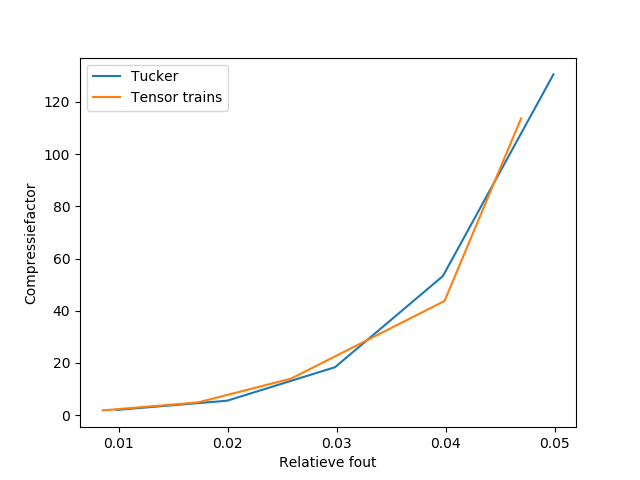
\includegraphics[width=\linewidth]{images/tensor_trains_st_hosvd_results_Indian_Pines.png}
  \caption{Indian Pines}
\end{subfigure}
\begin{subfigure}{0.48\textwidth}
  \centering
  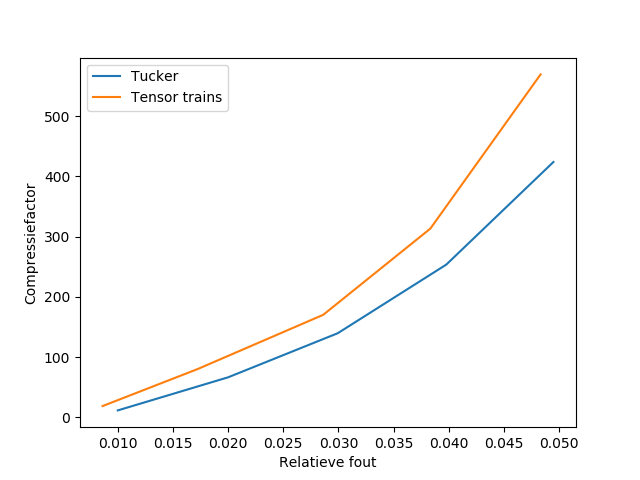
\includegraphics[width=\linewidth]{images/tensor_trains_st_hosvd_results_Cuprite.png}
  \caption{Cuprite}
\end{subfigure}
\\
\begin{subfigure}{0.48\textwidth}
  \centering
  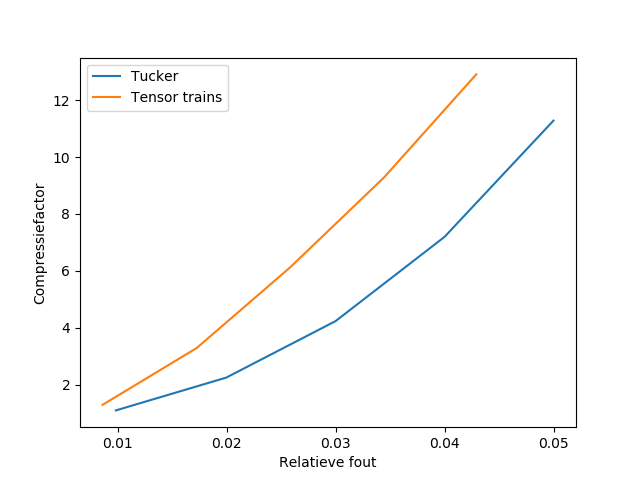
\includegraphics[width=\linewidth]{images/tensor_trains_st_hosvd_results_Pavia_Centre.png}
  \caption{Pavia Centre}
\end{subfigure}
\begin{subfigure}{0.48\textwidth}
  \centering
  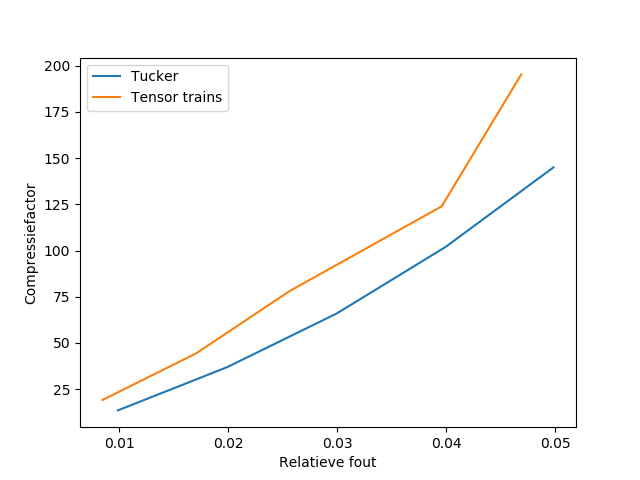
\includegraphics[width=\linewidth]{images/tensor_trains_st_hosvd_results_Mauna_Kea.png}
  \caption{Mauna Kea}
\end{subfigure}
\caption{Resultaten van de Tucker-decompositie (zonder hervorming, blauw) en tensor trains (oranje) voor verschillende datasets, na alleen het uitvoeren van de ST-HOSVD (dus zonder orthogonaliteitscompressie, quantisatie of encodering).}
\label{fig:tensor_trains_st_hosvd_results}
\end{figure}

\subsection{Eerste resultaten}

Analoog aan de vorige sectie, hebben we in figuur \ref{fig:tensor_trains_st_hosvd_results} de resultaten na alleen het uitvoeren van de ST-HOSVD vergeleken tussen tensor trains en de Tucker-decompositie (zonder hervorming). Bij Indian Pines, een kleine en minder belangrijke dataset, doen beide methoden het ongeveer even goed, terwijl in alle andere gevallen tensor trains betere resultaten geven. Het is dus zeker interessant om deze techniek verder te onderzoeken.

\subsection{Verdere uitwerking}

Zoals in hoofdstuk \ref{hoofdstuk:tucker} uitgebreid beschreven werd, moeten er bij het ontwikkelen van een volledig compressie-algoritme een aantal ontwerpkeuzes gemaakt worden. Aangezien we de meeste technieken hergebruiken, zullen we dit hier slechts kort bespreken:

\newpage
\begin{enumerate}
\item \textbf{Versnellen van de ST-HOSVD:}
\begin{enumerate}
\item \textbf{Modevolgorde:} Zoals eerder, de spectrale mode wordt eerst verwerkt, gevolgd door de spatiale modes in volgorde van dalende grootte.
\item \textbf{Versnellen van de SVD:} De SVD wordt berekend aan de hand van de methode met Gram-matrix, zolang deze werkelijk kleiner is dan de originele matrix. Bij de latere modes kan $n_{i+1} n_{i+2} \dots n_k$, het aantal te verwerken vectoren, kleiner zijn dan de dimensie van deze vectoren $r_{i-1} n_i$. In deze gevallen zullen we de SVD op de normale manier berekenen.
\end{enumerate}
\item \textbf{Orthogonaliteitscompressie:} Zoals eerder gebruiken we de methode met Householder-reflecties, aangezien deze een ideaal resultaat geven.

\newpage
\item \textbf{Quantisatie:}
\begin{enumerate}

\item \textbf{Kerntensor:} In figuur \ref{fig:tensor-trains-core-tensor-size} zien we dat de factormatrices bijna alle ruimte innemen bij een typische tensor train. Bijgevolg zullen we de kerntensor simpelweg niet quantiseren.

\begin{figure}[]
  \centering
  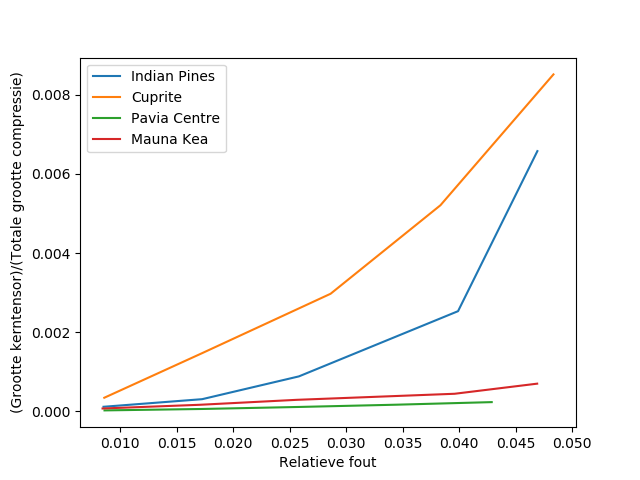
\includegraphics[scale=0.7]{images/tensor_trains_core_tensor_size.png}
  \caption{Het aandeel van de kerntensor in de compressie bij tensor trains, na alleen het uitvoeren van de ST-HOSVD.}
\label{fig:tensor-trains-core-tensor-size}
\end{figure}

\item \textbf{Factormatrices:} Zoals eerder, we gebruiken gelaagde quantisatie met norm-gebaseerde bit-aantal-selectie.
\end{enumerate}
\item \textbf{Encodering:} Zoals eerder, we zullen adaptieve encodering gebruiken zonder benaderende Huffman-codes.

\begin{figure}[]
  \centering
  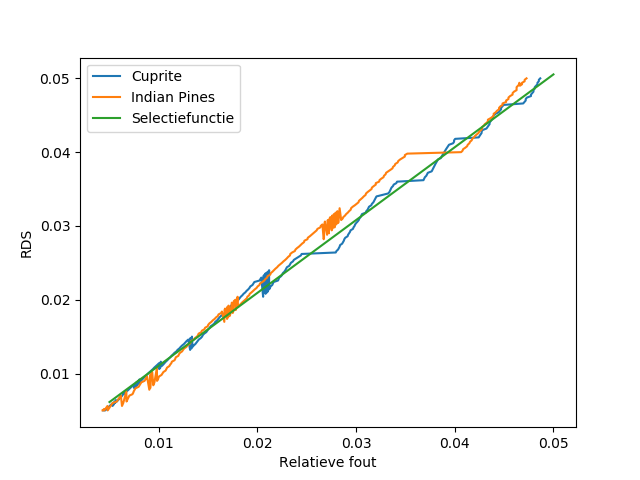
\includegraphics[scale=0.7]{images/filtered_sweep_points_tensor_trains_RDS.png}
  \caption{RDS-waarden van steekproefoptima en de RDS-selectiefunctie.}
\label{fig:filtered-sweep-points-tensor-trains-RDS}
\end{figure}

\begin{figure}[]
  \centering
  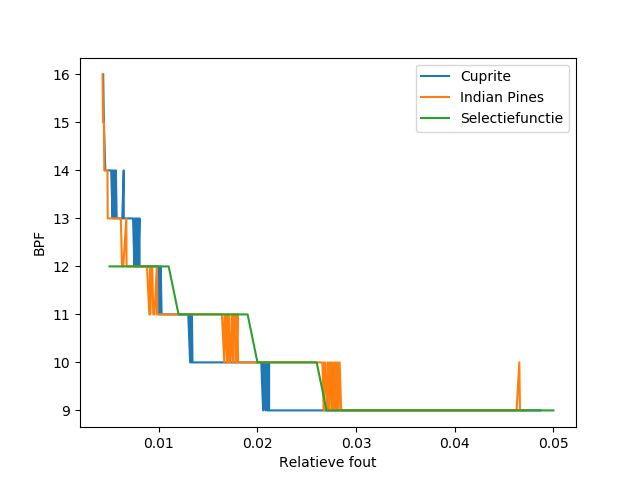
\includegraphics[scale=0.7]{images/filtered_sweep_points_tensor_trains_BPF.png}
  \caption{BPF-waarden van steekproefoptima en de BPF-selectiefunctie.}
\label{fig:filtered-sweep-points-tensor-trains-BPF}
\end{figure}

\item \textbf{Parameterselectie:} Aangezien de kerntensor niet meer gequantiseerd wordt, moeten alleen de RDS- en BPF-parameters afgesteld worden. Bij het verkennen van de parameterruimte beschouwen we de volgende domeinen: $RDS \in \{0.005, 0.0052, 0.0054, \dots, 0.05\}$ en $BPF \in \{16, 15, 14, \dots, 1\}$.
\begin{enumerate}

\item \textbf{Niet-adaptief:} Als we kijken naar de parameterwaarden die corresponderen met de steekproefoptima (Pareto-effici\"ente parametercombinaties), bekomen we figuren \ref{fig:filtered-sweep-points-tensor-trains-RDS} en \ref{fig:filtered-sweep-points-tensor-trains-BPF}. We kiezen de volgende selectiefuncties, op analoge wijze als in sectie \ref{sec:parameters}:
\begin{itemize}
\item $RDS = max(0.001, 0.986746*\text{kwaliteit} - 0.001199)$
\item $BPF = max(9, round(-132.505*\text{kwaliteit} + 13.048))$
\end{itemize}

\newpage
\item \textbf{Adaptief:} We zullen, zoals eerder, ook een adaptieve selectieprocedure uitwerken. Hierbij wordt de RDS weer vast gekozen aan de hand van de RDS-selectiefunctie en verlagen we de BPF-waarde (startend bij de waarde gekozen door de BPF-selectiefunctie) totdat de compressiefout de kwaliteitsparameter overschrijdt. Omdat er maar \'e\'en parameter adaptief gekozen wordt in plaats van twee, is deze procedure veel simpeler dan bij Tucker-gebaseerde compressie.\\

In figuren \ref{fig:parameter_functions_results_including_adaptive_Cuprite_tensor_trains} en \ref{fig:parameter_functions_results_including_adaptive_Indian_Pines_tensor_trains} tonen we opnieuw een vergelijking van compressie met (niet-)adaptieve parameterselectie en met optimale parameters uit de steekproef van ons onderzoek. We zien dat er voor Cuprite en Indian Pines weinig verschil is tussen het adaptieve en niet-adaptieve resultaat. We hebben ook gekeken naar grotere datasets, maar daar werkte de niet-adaptieve methode ook even goed, zonder de extra rekenkost, dus we zullen niet verder werken met adaptieve parameterselectie voor tensor trains.

\end{enumerate}
\end{enumerate}

\begin{figure}[H]
  \centering
  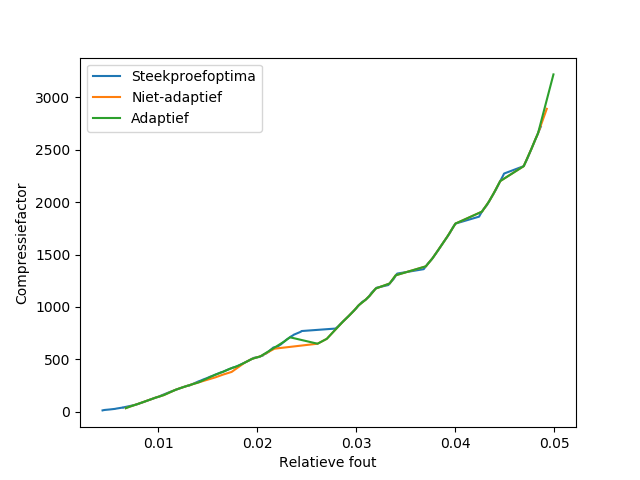
\includegraphics[scale=0.7]{images/parameter_functions_results_including_adaptive_Cuprite_tensor_trains.png}
  \caption{Resultaten van compressie met en zonder adaptieve parameterselectie voor Cuprite.}
  \label{fig:parameter_functions_results_including_adaptive_Cuprite_tensor_trains}
\end{figure}

\newpage
\begin{figure}[H]
  \centering
  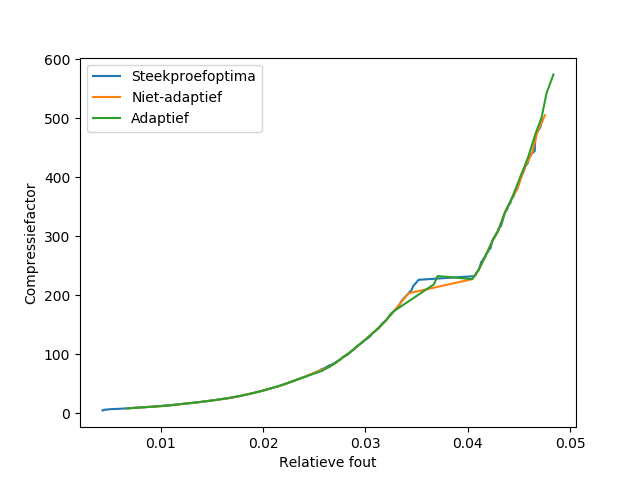
\includegraphics[scale=0.7]{images/parameter_functions_results_including_adaptive_Indian_Pines_tensor_trains.png}
  \caption{Resultaten van compressie met en zonder adaptieve parameterselectie voor Indian Pines.}
  \label{fig:parameter_functions_results_including_adaptive_Indian_Pines_tensor_trains}
\end{figure}
